% L43_P1_obs_student.tex
% Algebra 2  Lesson 4-3, Period 1 (Observation Day)
% Visual + structural reference: L35_P3_obs_student.docx (repo root)
%
% Structure (mirrors the DOCX exactly):
%   1. Title (centered, bold)
%   2. 3-row Objectives table (Math / Language / Essential Question)
%   3. Do Now              -- "Explore & Reason" (DOK-2 conceptual gateway)
%   4. Apply -- Make Sense and Persevere  -- #35 cylinders V/SA (DOK-2)
%   5. Performance Task    -- #36 Lupe carnival probability (DOK-2->3 model)
%   6. Name ___ line + Exit Ticket  -- #13 closure question + 2 reflection prompts
%
% Throughline (the spine the four problems collectively express):
%   "Domain restriction is the soul of a rational expression --
%    it survives even when factors cancel."

\documentclass[11pt]{article}
\usepackage[margin=0.75in]{geometry}
\usepackage{enumitem}
\usepackage{tabularx}
\usepackage{array}
\usepackage{amsmath}
\usepackage{amssymb}
\usepackage{tikz}
\usetikzlibrary{patterns}

\setlength{\parindent}{0pt}
\renewcommand{\arraystretch}{1.15}

\newcommand{\framedline}[1]{\underline{\hspace{#1}}}
\newcommand{\frameblank}{\underline{\hspace{4em}}}
% \writeline = invisible baseline strut (preserves the vertical writing room
% of a full-width line without rendering the underline). Used in place of
% \writeline so students see open white space, not ruled lines.
\newcommand{\writeline}{\rule[-2pt]{0pt}{12pt}}

\begin{document}

% =====================================================================
% TITLE
% =====================================================================
\begin{center}
{\Large\bfseries Lesson 4.3: Multiply and Divide Rational Expressions}
\end{center}

\vspace{0.3em}

% =====================================================================
% OBJECTIVES TABLE  (3 rows: Math Obj / Language Obj / Essential Q)
% Plain bordered table -- mirrors the DOCX header, no colored callout.
% =====================================================================
\noindent
\begin{tabularx}{\linewidth}{|>{\bfseries\raggedright\arraybackslash}p{1.55in}|X|}
  \hline
  Math Objectives &
    Identify the values that must be excluded from the domain of a
    rational expression. \par
    Simplify rational expressions by factoring and canceling common
    factors, then state the domain. \par
    Build and interpret rational expressions that arise from real-world
    ratios (geometry, probability, efficiency). \\ \hline
  Language Objective &
    Students will explain why a domain restriction must come from the
    \emph{original} denominator (not the simplified one), verbally and
    in writing, with the support of structured talk-time, models, and
    real-time scaffolding/questioning. \\ \hline
  Essential Question &
    What stays the same and what changes when we rewrite a rational
    expression in simplified form? \\ \hline
\end{tabularx}

\vspace{1em}

% =====================================================================
% DO NOW -- Explore & Reason  (10 min)
% Replaces the L35_P3_obs DOCX "Do Now" graph-match item.
% =====================================================================
\textbf{Do Now}

\vspace{0.3em}
Consider the following graph of the function $y = x + 2$.

\begin{center}
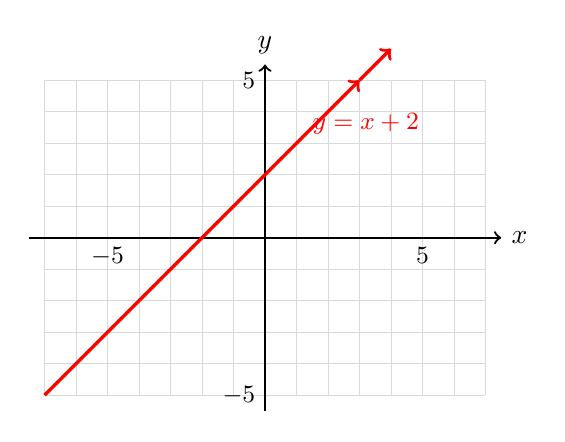
\begin{tikzpicture}[scale=0.4]
  \draw[very thin, gray!30] (-7,-5) grid (7,5);
  \draw[->, thick] (-7.5,0) -- (7.5,0) node[right] {$x$};
  \draw[->, thick] (0,-5.5) -- (0,5.5) node[above] {$y$};
  \foreach \x in {-5,5} \node[below] at (\x,0) {\small$\x$};
  \foreach \y in {-5,5} \node[left] at (0,\y) {\small$\y$};
  \draw[red, very thick, ->] (-7,-5) -- (3,5);
  \draw[red, very thick, ->] (3,5) -- (4,6);
  \node[red] at (3.2,3.6) {\small$y=x+2$};
\end{tikzpicture}
\end{center}

\textbf{A.} What is the domain of this function? \\
\writeline \\[6pt]
\writeline

\vspace{0.3em}
\textbf{B.} Sketch a function that resembles the graph, but \emph{restrict its domain to exclude} $x = 2$.

\begin{center}
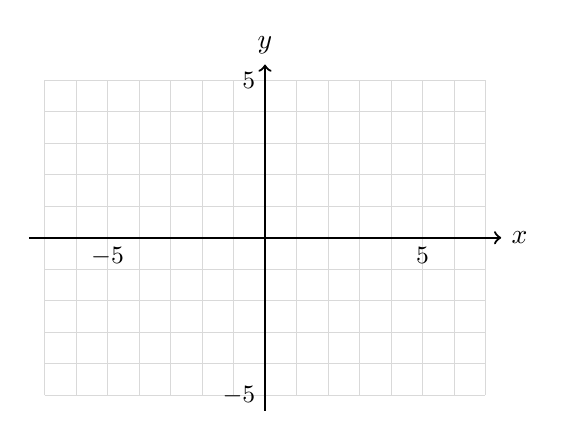
\begin{tikzpicture}[scale=0.4]
  \draw[very thin, gray!30] (-7,-5) grid (7,5);
  \draw[->, thick] (-7.5,0) -- (7.5,0) node[right] {$x$};
  \draw[->, thick] (0,-5.5) -- (0,5.5) node[above] {$y$};
  \foreach \x in {-5,5} \node[below] at (\x,0) {\small$\x$};
  \foreach \y in {-5,5} \node[left] at (0,\y) {\small$\y$};
\end{tikzpicture}
\end{center}

\vspace{0.3em}
\textbf{C.}\; \textbf{Use Structure.}\; What \emph{kind of function} might have a graph like the one you sketched in part B? Explain. \\
{\small\itshape Frame: ``The graph could come from a function whose denominator is \frameblank, because that makes $x = $ \frameblank\ excluded.''}\\
\writeline

\newpage

% =====================================================================
% APPLY -- Make Sense and Persevere  (15 min)
% Mirrors L35_P3_obs DOCX "Apply -- Make Sense and Persevere"
% Source: Savvas Practice #35 (cylinder A vs B, V/SA ratio comparison)
% =====================================================================
\textbf{Apply -- Make Sense and Persevere}

\vspace{0.3em}
An engineering firm wants to construct a cylindrical structure that will
\emph{maximize the volume for a given surface area}. Compare the ratios of
the volume to surface area of each of the cylindrical structures shown,
using the following formulas for volume and surface area of cylinders.
\[
V = \pi r^{2} h \qquad SA = 2\pi r h + 2\pi r^{2}
\]

\begin{center}
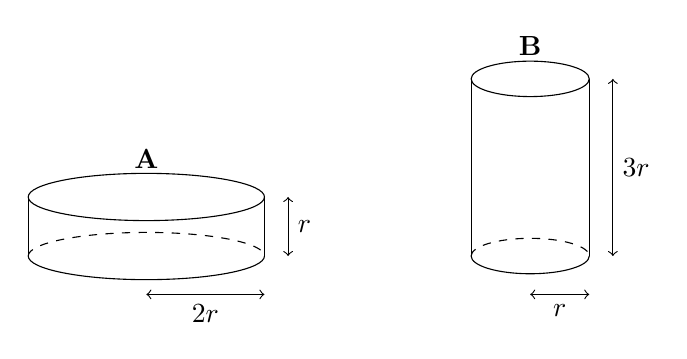
\begin{tikzpicture}[scale=0.75]
  % Cylinder A: radius 2r, height r  (wide and short -- per Savvas SE 4-3 #35)
  \begin{scope}[shift={(0,0)}]
    \draw (-2,0) -- (-2,1);
    \draw (2,0) -- (2,1);
    \draw (0,1) ellipse (2 and 0.4);
    \draw (-2,0) arc (180:360:2 and 0.4);
    \draw[dashed] (-2,0) arc (180:0:2 and 0.4);
    \draw[<->] (0,-0.65) -- (2,-0.65) node[midway,below] {$2r$};
    \draw[<->] (2.4,0) -- (2.4,1) node[midway,right] {$r$};
    \node at (0,1.65) {\textbf{A}};
  \end{scope}
  % Cylinder B: radius r, height 3r  (narrow and tall -- per Savvas SE 4-3 #35)
  \begin{scope}[shift={(6.5,0)}]
    \draw (-1,0) -- (-1,3);
    \draw (1,0) -- (1,3);
    \draw (0,3) ellipse (1 and 0.3);
    \draw (-1,0) arc (180:360:1 and 0.3);
    \draw[dashed] (-1,0) arc (180:0:1 and 0.3);
    \draw[<->] (0,-0.65) -- (1,-0.65) node[midway,below] {$r$};
    \draw[<->] (1.4,0) -- (1.4,3) node[midway,right] {$3r$};
    \node at (0,3.55) {\textbf{B}};
  \end{scope}
\end{tikzpicture}
\end{center}

\vspace{0.3em}
\textbf{a.} Calculate the ratio of volume to surface area for cylinder A. \\
\writeline \\[8pt]
\writeline \\[8pt]
\writeline \\[8pt]
\writeline

\vspace{0.3em}
\textbf{b.} Calculate the ratio of volume to surface area for cylinder B. \\
\writeline \\[8pt]
\writeline \\[8pt]
\writeline \\[8pt]
\writeline

\vspace{0.3em}
\textbf{c.} Which of these cylinders has a greater ratio of volume to surface area? \emph{What does that mean about the design?} \\
{\small\itshape Frame: ``Cylinder \frameblank\ has the greater ratio because \frameblank, which means a designer who wants the most volume per unit of material should pick \frameblank.''}\\
\writeline \\[8pt]
\writeline \\[8pt]
\writeline

\newpage

% =====================================================================
% PERFORMANCE TASK -- Model with Mathematics  (20 min)  -- DOK-3 SPINE
% Mirrors L35_P3_obs DOCX "Performance Task" (Venetta deli).
% Source: Savvas Practice #36 (Lupe carnival probability ratio)
% Scaffolded into A/B/C parts to match Venetta's build->simplify->interpret arc.
% =====================================================================
\textbf{Performance Task}

\vspace{0.3em}
Lupe designed a carnival game that involves tossing a beanbag into the
box shown. To win a prize, the beanbag must fall inside the
\textbf{black rectangle}. The probability of winning is equal to the
ratio of the area of the black rectangle to the total area of the face
of the box shown.

\begin{center}
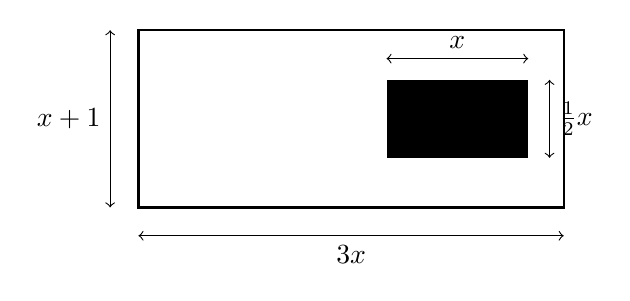
\begin{tikzpicture}[scale=0.9]
  % Outer rectangle: width 3x, height x+1
  \draw[thick] (0,0) rectangle (6,2.5);
  % Inner black rectangle: width x, height (1/2)x
  \fill[black] (3.5,0.7) rectangle (5.5,1.8);
  % Dimension labels for outer
  \draw[<->] (0,-0.4) -- (6,-0.4) node[midway,below] {$3x$};
  \draw[<->] (-0.4,0) -- (-0.4,2.5) node[midway,left] {$x+1$};
  % Dimension labels for inner
  \draw[<->] (3.5,2.1) -- (5.5,2.1) node[midway,above] {$x$};
  \draw[<->] (5.8,0.7) -- (5.8,1.8) node[midway,right] {$\tfrac{1}{2}x$};
\end{tikzpicture}
\end{center}

\vspace{0.3em}
\textbf{A.}\; Write the rational expression for the probability of winning. \emph{Show what you used for the numerator and denominator.} \\
\writeline \\[8pt]
\writeline \\[8pt]
\writeline \\[8pt]
\writeline

\vspace{0.3em}
\textbf{B.}\; Simplify the expression. State the domain restrictions and explain what they mean \emph{in this physical situation} (the carnival box). \\
{\small\itshape Frame: ``The simplified expression is \frameblank. The value $x = $ \frameblank\ is excluded because \frameblank.''}\\
\writeline \\[8pt]
\writeline \\[8pt]
\writeline \\[8pt]
\writeline \\[8pt]
\writeline

\vspace{0.3em}
\textbf{C.}\; Suppose Lupe builds the game with $x = 4$ feet. What is the probability that a randomly thrown beanbag wins? \emph{Would you say this is a fair carnival game? Why or why not?} \\
{\small\itshape Frame: ``When $x = 4$, the probability is \frameblank. I think the game is \frameblank\ because \frameblank.''}\\
\writeline \\[8pt]
\writeline \\[8pt]
\writeline \\[8pt]
\writeline

\newpage

% =====================================================================
% EXIT TICKET (5 min) -- forced onto its own page (page 4) so students
% have generous writing room and the page can be torn off / collected.
% Mirrors L35_P3_obs DOCX exit: short conceptual prompt + 2 reflection lines.
% Source: Savvas Practice #14 (Use Appropriate Tools, DOK-2). Swapped from
% the original #13 (HOT, DOK-3) to avoid a second DOK-3 spine in the
% period (#36-partC-evaluate-fairness is the spine). #14 keeps the
% throughline ("domain restrictions are necessary") in summary-exit form.
% =====================================================================
\textbf{Name} \framedline{4.5in}

\vspace{0.8em}
\textbf{Exit Ticket}

\vspace{0.5em}
\textbf{Use Appropriate Tools.}\; Explain why domain restrictions are necessary to show that the rational expressions $\dfrac{-6x^{2}+21x}{3x}$ and $-2x+7$ are equivalent. What is true about the graphs at $x = 0$, and why? \\
\writeline \\[8pt]
\writeline \\[8pt]
\writeline \\[8pt]
\writeline

\vspace{0.4em}
{\small\itshape You may use any of these sentence frames if they help:}
\begin{itemize}[leftmargin=2em, itemsep=2pt, topsep=2pt]
  \item ``At $x = $ \frameblank, the original expression $\dfrac{-6x^{2}+21x}{3x}$ is undefined because \frameblank.''
  \item ``The graph of $\dfrac{-6x^{2}+21x}{3x}$ has a \frameblank\ at $x = 0$, but the graph of $-2x+7$ does not.''
  \item ``Without the domain restriction, the two expressions are not \frameblank.''
\end{itemize}

\vspace{1em}
\textbf{What is something you learned today?} \\
\writeline \\[8pt]
\writeline \\[8pt]
\writeline \\[8pt]
\writeline

\vspace{0.5em}
\textbf{What is something you liked about this lesson?} \\
\writeline \\[8pt]
\writeline \\[8pt]
\writeline \\[8pt]
\writeline

\end{document}
